% kapitel3.tex
\chapter{Implementierung} \label{sec:alg}
Für das in Python implementierte RAD-Sequencing-Tool, NodeRAD, wurde zur Workflowintegration das Workflow Management System Snakemake verwendet ~\cite{koester_2012_1, koester_2012_2}. Die einzelnen Analyseschritte werden dabei über Regeln abgebildet. Für jede Regel können neben dem zu verwendenden Script oder Shell-Kommando sowie den Pfadangaben für In- und Output auch zusätzliche Optionen festgelegt werden. Dazu gehören beispielsweise Angaben zu Parametern bzw. Argumenten für die verwendeten Tools, Pfadangaben für Log-Dateien oder die Anzahl der zu verwendenden Threads. \\

Als Input benötigt der Workflow eine Datei im FASTQ-Format (siehe Kap. \ref{subsec:fastq}), welche die single-end Reads der verschiedenen Individuen mit ihren Identifikationsbezeichnungen, der Basensequenz und Angaben zur  Basenqualität enthält. Des Weiteren wird eine Tabelle im tsv-Format benötigt, in der die Zuordnung der Probennamen zu den Individuen und ihren Barcode-Sequenzen definiert ist. Nach dem Preprocessing, der Qualitätskontrolle der Reads und dem Sequenzalignment erfolgt die RAD-Seq-Analyse durch NodeRAD. Hierbei werden die Wahrscheinlichkeiten der Allele-Fractions und der möglichen Loci bestimmt. Die Loci mit der höchsten Wahrscheinlichkeit werden schließlich mit den Sequenzen ihrer Allele in einer Datei im Variant Call Format (VCF) ausgegeben.

\section{Preprocessing} \label{sec:preproc}

Im Preprocessing werden durch das Tool Cutadapt ~\cite{martin_2011} die Reads jedes Individuums anhand ihrer Barcodesequenzen identifiziert und extrahiert (Demultiplexing). Hiernach werden die Barcodesequenzen entfernt (Trimming) und die Reads jedes Individuums in separaten Dateien im FASTQ Format abgelegt. \\
Im Anschluss an das Trimming erfolgt eine Qualitätskontrolle durch das Tool FastQC  ~\cite{andrews_2012}. Dabei werden einige allgemeine Statistiken zu den Rohdaten der Reads generiert, wie beispielsweise zur Basenqualität, zum GC-Gehalt, dem Anteil an Duplikaten oder überrepräsentierten Sequenzen. Durch das Tool MultiQC ~\cite{ewels_2016} wird aus diesen Statistiken und den Log-Dateien von Cutadapt ein Report im HTML-Format mit diversen Plots zur Veranschaulichung erstellt.

\section{Edit-Distanzen} \label{sec:edit}

Für die spätere Konstruktion eines Graphen basierend auf den Edit-Distanzen zwischen den Readsequenzen wird für jedes Individuum zunächst ein Sequenzalignment (vgl. Kap. \ref {subsec:samformat}) mit Hilfe des Tools Minimap2 ~\cite{li_2018} erstellt. Hierbei werden alle Readsquenzen paarweise mit einander verglichen. Das Ergebnis des Mappings wird im SAM/BAM-Format ~\cite{li_2009} ausgegeben und enthält neben den Angaben zur Query- und Referenzsequenz auch den CIGAR-String sowie den NM-Tag mit den Edit-Distanzen. Der CIGAR-String und der NM-Tag definieren wichtige Kanteneigenschaften des späteren Graphen. \\

\section{Konstruktion des Graphen} \label{sec:graph}
\subsection{Knoten des Graphen} \label{subsec:nodes}
NodeRAD benötigt als Input zu jedem Individuum die getrimmten single-end Reads sowie das Sequenzalignment. Zunächst wird daraus für jedes Individuum ein eigener, gerichteter Graph $ G $ mit $ G = (V,E) $ erstellt. Seine Knoten, $ V $, werden durch die einzelnen Reads repräsentiert. Entsprechend ergeben sich die Knoteneigenschaften aus den Daten der Reads, diese werden den FASTQ-Dateien nach Ausführung von Cutadapt (siehe \ref{sec:preproc}) entnommen. Die Kanten, $ E $, zwischen den Knoten ergeben sich aus dem Vergleich ihrer Sequenzen im Rahmen des Sequenzalignments mittels Minimap2 (siehe \ref{sec:edit}).\\

Zusätzlich entnimmt NodeRAD der Konfigurationsdatei des Workflows einige Konstanten und Grenzwerte für die späteren Berechnungen. Zu den Konstanten gehören die verschiedenen Mutationsraten und Heterozygotiewahrscheinlichkeiten für Substitutionen, Insertionen und Deletionen, die Ploidie des Chromosomensatzes der untersuchten Spezies. Diese werden im Script \lstinline|noderad_main.py| im Graphen als Grapheigenschaften abgelegt. Als konfigurierbare Grenzwerte gibt es für NodeRAD einen Schwellenwert \lstinline|edit-distance-graph| für die maximal zulässige Edit-Distanz, bei der zwei Knoten noch durch eine Kante verbunden werden sowie Schwellenwerte zum Filtern selten vorkommender Sequenzen \linebreak (\lstinline|treshold-seq-noise|) ab einer bestimmten Clustergröße (\lstinline|treshold-cluster-size|), die als Hintergrundrauschen nicht in der Berechnung Berücksichtigung finden sollen. \\

Zur Konstruktion des Graphen wird die Python-Library graph-tool ~\cite{peixoto_2014} genutzt. Die Knoten werden aus den FASTQ-Daten der getrimmten Reads mittels SeqIO aus der Library Biopython ~\cite{cock_2009_1} ausgelesen und im Graphen mit den Knoteneigenschaften ihrer Basensequenz, einer internen ID sowie Angaben zur Basenqualität abgelegt. Die Codierung des Qualitystrings der Reads variiert je nach verwendeter Plattform. Daher wird er durch SeqIO ausgelesen und für jede Base in ein einheitliches Maß, den Phred Quality Score, decodiert ~\cite{cock_2009_2}.
Für jeden Knoten werden die Vektoren mit den Phred Qualitiy Scores der Basen als Knoteneigenschaft gespeichert. \\

\subsection{Kanten des Graphen} \label{subsec:edges}
Die Kanten des Graphen definieren sich durch die mittels Minimap2 erzeugten Sequenzalignments (vgl. Kap. \ref{sec:edit}). Jedes Alignment zweier Reads entspricht im Graphen einer gerichteten Kante $e = (source,\; target)$, die den Vergleich der Query- zur Referenzsequenz repräsentiert. Sie verbindet somit zwei der zuvor aus der FASTQ-Daten erzeugten Knoten. Das Auslesen des SAM/BAM-Formats des Alignmentfiles erfolgt mit Hilfe der Python-Library pysam ~\cite{pysam}. Dabei werden die Edit-Distanzen aus dem NM-Tag genutzt, um nur Kanten in den Graphen aufzunehmen, die unterhalb des durch die Konfigurationsdatei festgelegten Grenzwertes \lstinline|threshold_max_edit_distance| liegen. Neben den Edit-Distanzen wird als weitere Kanteneigenschaft der zu Tupeln decodierte CIGAR-String hinzugefügt. Zusätzlich kann zur Kontrolle oder für eine spätere Verwendung auch der cs-Tag (Kap. \ref{subsec:samformat}) als Kanteneigenschaft gespeichert werden, falls bei Minimap2 die Option zur Erzeugung des cs-Tags aktiviert wurde. Die CIGAR-Tupel werden durch pysam aus dem CIGAR-String (Kap. \ref{subsec:samformat}) geparsed. Hierbei handelt es sich um eine Liste von Tupeln, die jeweils aus Integer-Wertepaaren bestehen. Der erste Wert jedes Tupels gibt die spezifische Operation des Matches oder Mismatches an. So entspricht beispielsweise ein Wert von $ 7 $ oder $ 0 $ einem Match und ein Wert von $ 2 $ einer Deletion. Der zweite Werte jedes Tupels gibt die Anzahl der Basen an, die von der entsprechenden Operation betroffen sind. Die CIGAR-Tupel werden für die Berechnung der Likelihood zwischen zwei Knoten benötigt (Kap. \ref{phmm_minimap}). Dies erfolgt zum einen zur Bestimmung der Likelihood der Allele-Fractions (Kap. \ref{subsec:lh_allele}) und zum anderen, um die Likelihood der Loci-Kombinationen zu ermitteln. \\

Nach Abschluss der Graphkonstruktion werden für jedes Individuum Anzahl der Knoten und Kanten des Graphen in den Log-Dateien festgehalten. Als optionaler Output können über die Konfigurationsdatei und die Snakemake-Regel \lstinline|rule noderad| auch die detaillierten Graphinformationen sowie eine Visualisierung des Graphen ausgegeben werden. Die Graphinformationen wie Knoten, Kanten und ihre Eigenschaften können dabei im GraphMl-, DOT-, GML- oder im binären gt-Format gespeichert werden. Die graphische Darstellung wird als pdf-Datei ausgegeben. \\

\subsection{Bestimmung der Zusammenhangskomponenten} \label{subsec:comp}

Die Bestimmung der Zusammenhangskomponenten erfolgt durch graph-tool ~\cite{docs_graph_tool}. Die Indexnummer jeder Zusammenhangskomponente wird den in ihr enthaltenen Knoten als Knoteneigenschaft hinzugefügt. Zusammenhangskomponenten mit mehr als einem Knoten  werden als neuer eigenständiger Graph initialisiert und in einer Liste abgelegt. Hierfür wird aus dem Graphen für jede Komponente eine gefilterte Sicht erzeugt, die als neues Graph-Object gespeichert wird. \\

\begin{figure}[H]
	\begin{center}
		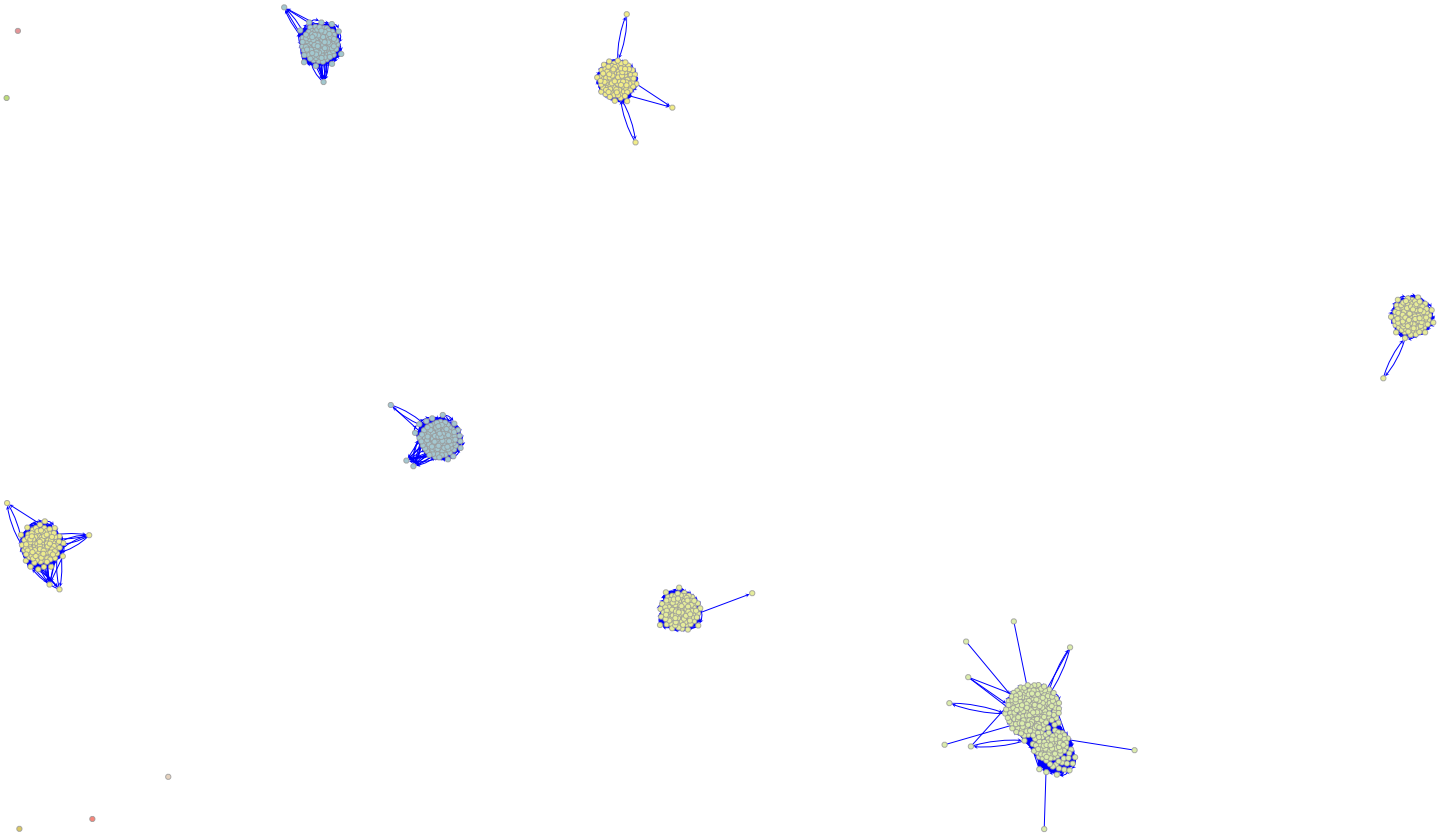
\includegraphics[width=0.8\textwidth]{bilder/components_all_5.png}
		\caption{Ausschnitt einiger Zusammenhangskomponenten des Gesamtgraphen }
		\label{fig:all_comp} 
	\end{center}
\end{figure}

Da alle weiteren Schritte des Algorithmus jeweils auf den einzelnen Komponenten durchgeführt werden, kann durch die Verwendung einer Liste von Graphen im Folgenden eine einfachen Iteration über die Komponenten ausgeführt werden, ohne dass der Filtervorgang über alle Knoten jeder Komponente wiederholt werden muss. Zudem ermöglicht diese Datenstruktur eine effizientere Traversierung und Suche innerhalb der Zusammenhangskomponente, ohne dass für jede Komponente der gesamte Graph betrachtet werden muss. Der ursprüngliche Graph wird anschließend entfernt, um Arbeitsspeicher freizugeben. \\

In der Log-Datei wird die Anzahl der Knoten aller Zusammenhangskomponenten als Histogramm festgehalten. Ebenso wird dort für alle Komponenten mit mehr als einem Element die Anzahl ihrer Knoten, Kanten und Eigenschaften aufgelistet.\\

Über die Konfigurationsdatei und die Snakemake-Regel \lstinline|noderad| können optional auch für die Zusammenhangskomponenten jeweils Visualisierungen (siehe \autoref{fig:comp}) und detaillierte Graphinformationen in den oben genannten Formaten des Graphen (Kap. \ref{subsec:edges}) ausgegeben werden. \\

\begin{figure}[H]
	\subfigure{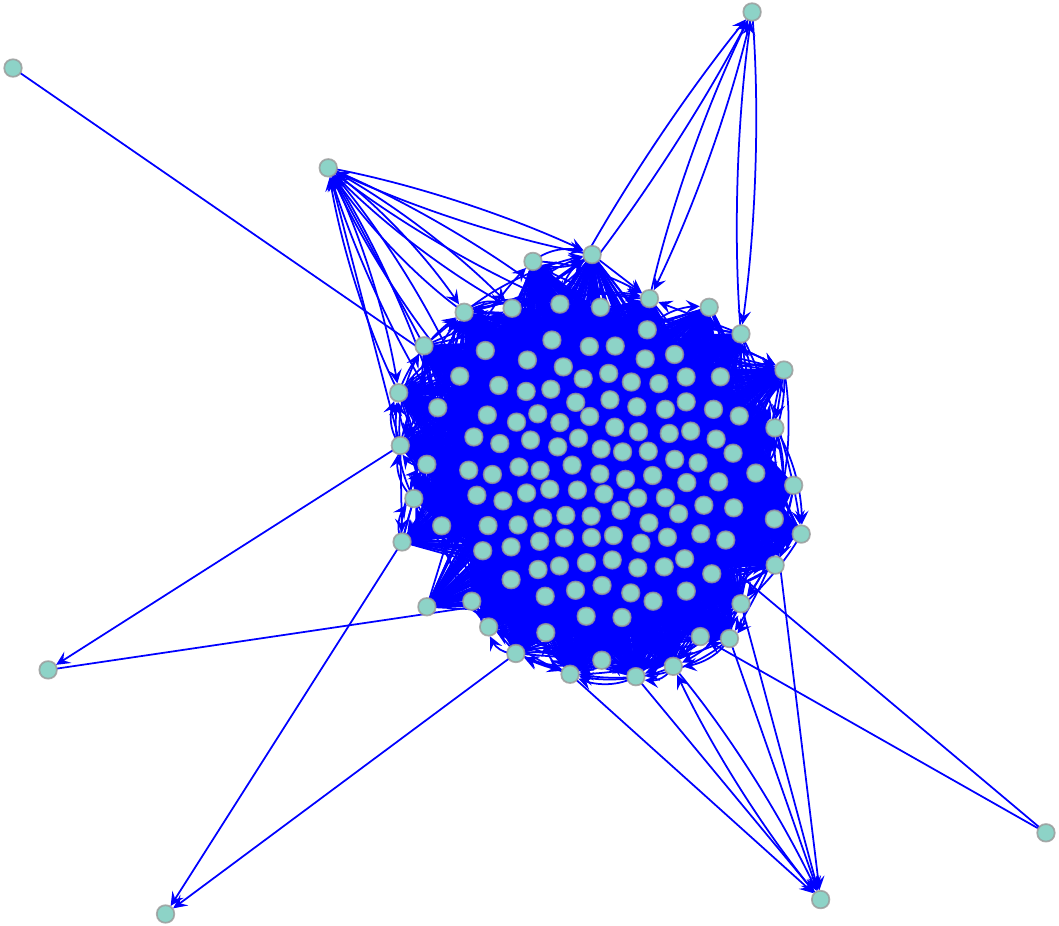
\includegraphics[width=0.49\textwidth]{bilder/components_1.png}}
	\subfigure{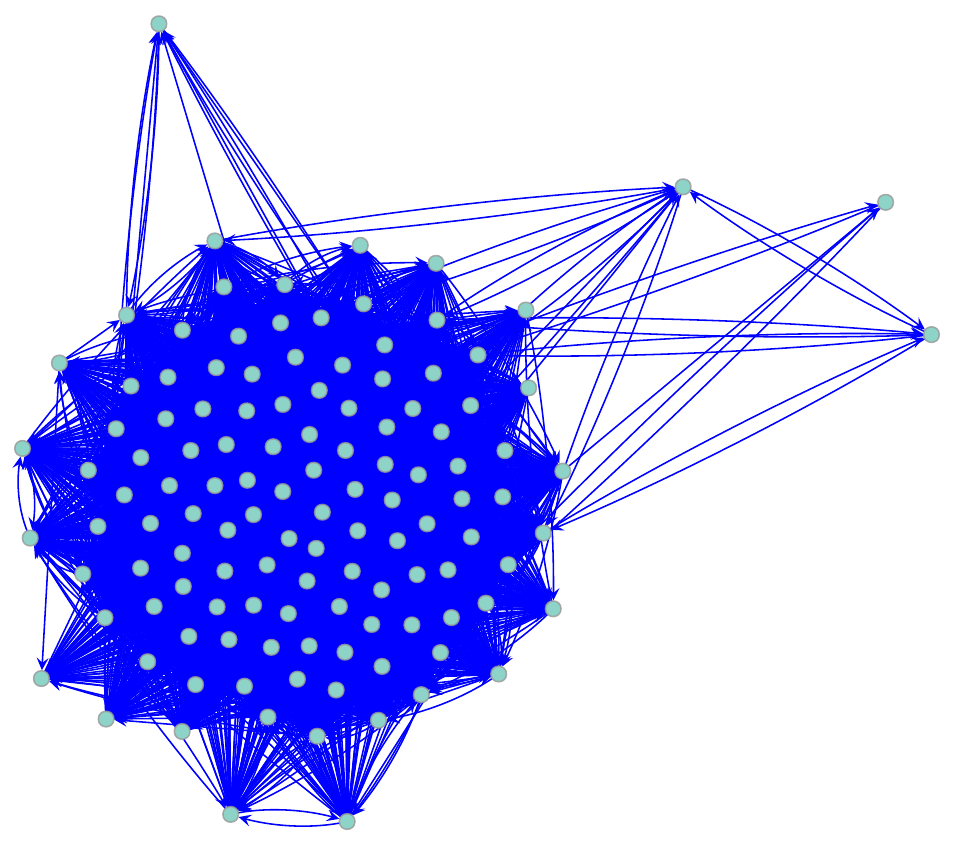
\includegraphics[width=0.49\textwidth]{bilder/components_4.png}}
	\caption{Beispiele einzelner Zusammenhangskomponenten}
	\label{fig:comp}
\end{figure}

Zudem kann optional auch der gesamte Graph mit den Komponentenindizes als Knoteneigenschaften gespeichert werden. In der visuellen Darstellung werden dort seine Knoten entsprechend der zugehörigen Zusammenhangskomponente eingefärbt (siehe \autoref{fig:all_comp}).\\

\section{Bestimmung der Allele-Fractions mit maximaler Likelihood} \label{sec:max_lh_allele}
\subsection{Bestimmung der Kandidatenallele und ihrer möglichen Häufigkeitsverteilung} \label{subsec:cand_allele}

Die einzelnen Zusammenhangskomponenten repräsentieren einen oder mehrere Loci. Alle weiteren Berechnungen aus diesem und den folgenden Kapiteln ~\ref{sec:max_lh_loci} und ~\ref{sec:vcf} werden für jede Komponente einzeln durchgeführt, dabei sollen die wahrscheinlichsten Allelsequenzen und die dazugehörigen Loci identifiziert werden. Die hierfür implementierten Funktionen finden sich im Modul \lstinline|likelihood_operations.py|. \\

Zunächst werden mit der Funktion \lstinline|get_candidate_alleles()| aus dem Modul \linebreak \lstinline|likelihood_operations.py| die Allelsequenzen ermittelt, die in der Zusammenhangskomponenten vorkommen. Für deterministischere Ergebnisse werden diese als lexikographisch sortierte Liste erzeugt. Übersteigt die Größe eines Clusters, d.h. die Knotenanzahl einer Zusammenhangskomponenten, den in der Konfigurationsdatei als \lstinline|treshold-cluster-size| festgelegten Grenzwert, so wird von allen vorkommenden Sequenzen des Clusters zunächst die absolute Häufigkeit bestimmt. Anschließend werden nur diejenigen Sequenzen lexikographisch sortiert zurückgegeben, die den \lstinline|treshold-seq-noise| Schwellenwert aus der Konfigurationsdatei überschreiten. Dies dient dazu, bei großen Clustern Komplexität und Rechenaufwand zu reduzieren, da davon auszugehen ist, dass innerhalb eines großen Clusters echte Varianten einer Sequenz mehrfach vorkommen, wohingegen Artefakte und Sequenzierfehler eher vereinzelt auftreten. Dieses sog. Rauschen kann durch Anpassung der Schwellwerte in der Konfigurationsdatei herausgefiltert werden. Da bei kleineren Clustern auch einmalig registrierte Varianten einer Sequenz von Bedeutung sein können, soll der Filtervorgang erst ab einer einstellbaren Clustergröße durchgeführt werden. \\

Aus der so erzeugten Liste lexikographisch sortierter Kandidatenallele $ A_{cand} $ der Länge $ n_{cand} $ sollen nun die möglichen Häufigkeitsverteilungen in Abhängigkeit von der Ploidie bestimmt werden. Hierzu muss zunächst die aufgrund der Ploidie tatsächlich zu erwartende Anzahl von Allelen $n_{alleles}$ bestimmt werden. Dies geschieht durch die Funktion \lstinline|get_max_parsimony_n_alleles()| in \lstinline|likelihood_operations.py|. Dadurch werden unnötige bzw. nicht mögliche Allelkombinationen eingespart und in der weiteren Berechnung nicht berücksichtigt. Ist die Ploidie $ \phi $ höher als die Anzahl der Kandidatenallele, so muss es mindestens genauso viele und bei Homozygotie auch mehrfach vorkommende Allele geben, damit die Ploidie erfüllt werden kann. Es muss also gelten $ n_{alleles} = \phi $. Wurden dagegen mehr Allele beobachtet als aufgrund der Ploidie möglich sind und die Ploidie ist Teiler von $n_{cand}$, so können alle beobachteten Allele auch tatsächlich vorkommen, da die Zusammenhangskomponente auch mehrere Loci enthalten kann. Es gilt dann also $ n_{alleles} = n_{cand} $. Ist dagegen die Anzahl der beobachteten Allele höher als die Ploidie, aber nicht ganzzahlig durch die Ploidie teilbar, so muss die Anzahl der Allele entsprechend erhöht werden. Das heißt, es müssen tatsächlich so viele Allele vorkommen, dass eine korrekte Ploidie erreicht wird, dass also die Ploidie eine Teiler von $ n_{alleles} $ wird. Die Anzahl der Allele muss also um die Ploidie abzüglich des Restes aus der Restdivision erhöht werden und es gilt $ n_{alleles} = n_{cand} + \phi - (n_{cand} \mod \phi)$. \\

Mit Hilfe der tatsächlich zu erwarteten Anzahl von Allelen $ n_{alleles} $ können nun alle Kombinationen möglicher Häufigkeitsverteilungen der Allele bestimmt werden (Funktion \linebreak \lstinline|get_candidate_vafs()| im Modul \lstinline|likelihood_operations.py|). Diese Häufigkeitsverteilungen werden auch als Allele-Fractions bezeichnet. Hierfür werden zunächst alle möglichen Allelkombinationen ermittelt. Dies erfolgt nach dem Urnenmodell unter Auswahl von $ n_{alleles} $ Elementen mit Zurücklegen aus insgesamt $ n_{cand} $ verschiedenen Elementen und ohne Berücksichtigung der Reihenfolge. Dadurch berechnet sich die Anzahl möglicher Kombination nach \eqref{eqn:3-12} aus dem  Binomialkoeffizienten der $k$-ten Ordnung aus $ n $ Elementen mit Zurücklegen ~\cite{tb_stat,bronst}.
\begin{equation} \label{eqn:3-12}
\tag{3-12}
\binom{n + k - 1}{k} = \frac{(n+k-1)!}{(n-1)!\, \cdotp k!} = \frac{(n_{alleles}+n_{cand}-1)!}{(n_{alleles}-1)!\, \cdotp n_{cand}!} 
\end{equation}

Die Allelkombinationen werden mit Hilfe der Funktion  \lstinline|combinations_with_replacement| aus der Python-Library \lstinline|itertools| erzeugt \cite{itertools}.\\
\\
\definecolor{light-gray}{gray}{0.93}
\fcolorbox{black}{light-gray}{
	\parbox{\textwidth}{
		\vspace{0.5cm}
		\textbf{Beispiele möglicher Allelkombinationen:} \\	
		\\	
		$ ploidy = 2, n_{cand} = 2, n_{alleles} = 2$: \\
		{[(0, 0), (0, 1), (1, 1)]}\\
		\\
		$ ploidy = 2, n_{cand} = 3, n_{alleles} = 4$: \\
		{[(0, 0, 0, 0), (0, 0, 0, 1), (0, 0, 0, 2), (0, 0, 1, 1), (0, 0, 1, 2), (0, 0, 2, 2), (0, 1, 1, 1), (0, 1, 1, 2), (0, 1, 2, 2), (0, 2, 2, 2), (1, 1, 1, 1), (1, 1, 1, 2), (1, 1, 2, 2), (1, 2, 2, 2), (2, 2, 2, 2)]}
		\\
	}}\\


Für jedes Allel $a_{i}$ können im Anschluss aus seinen absoluten Häufigkeiten $H_{a_{i}}$ innerhalb jeder Allelkombination die relativen Häufigkeiten $h_{a_{i}}$ nach \eqref{eqn:3-13} bestimmt werden. 
\begin{equation} \label{eqn:3-13}
\tag{3-13}
h_{a_{i}} = \frac{H_{a_{i}}} {n_{alleles}}
\end{equation}
\\		
\fcolorbox{black}{light-gray}{
	\parbox{\textwidth}{
		\vspace{0.5cm}
		\textbf{Beispiele möglicher Allele-Fractions:} \\	
		\\	
		$ ploidy = 2, n_{cand} = 2, n_{alleles} = 2$: \\
		{[1.0, 0.0]}, {[0.5, 0.5]}, {[0.0, 1.0]} \\
		\\
		$ ploidy = 2, n_{cand} = 3, n_{alleles} = 4$: \\
		{[1.0, 0.0, 0.0]}, {[0.75, 0.25, 0.0]}, {[0.75, 0.0, 0.25]}, {[0.5, 0.5, 0.0]}, {[0.5, 0.25, 0.25]}, {[0.5, 0.0, 0.5]}, {[0.25, 0.75, 0.0]}, {[0.25, 0.5, 0.25]}, {[0.25, 0.25, 0.5]}, {[0.25, 0.0, 0.75]}, {[0.0, 1.0, 0.0]}, {[0.0, 0.75, 0.25]}, {[0.0, 0.5, 0.5]}, {[0.0, 0.25, 0.75]}, {[0.0, 0.0, 1.0]}
		\\
}}
\linebreak 

\subsection{Berechnung der Likelihoods der Allele anhand der Allele-Fractions} \label{subsec:lh_allele}

In diesem Kapitel soll diejenige Allel-Fraction bestimmt werden, welche die beobachteten Reads am besten erklärt (vgl. Kap. \ref{subsec:sol_allele_lh}). Für jeden Read wird dafür zunächst die Wahrscheinlichkeit bestimmt, dass der Read durch Sequenzierfehler aus einem der Kandidatenallele entstanden ist. Hiernach wird für jeden Read die Wahrscheinlichkeit errechnet, diesen anhand einer gegebenen Allele-Fraction zu beobachten. Diese Berechnungen werden für alle Allele-Fractions durchgeführt. Aus der so gewonnenen Lösungsmenge wird die Allel-Fraction mit der höchsten Likelihood für die spätere Zuordnung der Loci (Kap. \ref{sec:max_lh_loci}) ausgewählt. \\ 

Zunächst wird in der Funktion \lstinline|get_allele_likelihood_read()| eine Kante zwischen dem betrachteten Read und dem Kandidatenallel gesucht. Während der Ausführung werden die Sequenzen und Likelihoods der bereits gefundenen Read-Kandidatenallel-Paare in einem Dictionary abgelegt. Als Key wird dabei das Tupel aus Read- und Allelsequenz verwendet, die berechnete Likelihood wird als Value eingetragen. Dies ermöglicht eine schnellere und effizientere Suche einer passenden Kante. \\

Existiert ein Read-Kandidatenallel-Paar noch kein Eintrag im Dictionary, so werden zuerst alle ausgehenden Nachbarn des Reads hinsichtlich ihrer in den Knoteneigenschaften abgelegten Sequenz geprüft. Besitzt einer der ausgehenden Nachbarknoten die Sequenz des Kandidatenallels, so wird die Likelihood durch \lstinline|get_alignment_likelihood()| berechnet (Algorithmus \ref{alg:lh_read}), ein entsprechender Eintrag im Dictionary angelegt und die Likelihood zurückgegeben.\\

Gibt es keine solche Kante, die vom Read zu einem Knoten mit Kandidatenallelsequenz führt, so wird geprüft, ob es eine Kante in umgekehrter Richtung gibt. Hierfür werden nun alle eingehenden Nachbarn des Reads betrachtet. Findet sich unter ihnen ein Knoten mit der gesuchten Kandidatenallelsequenz, so wird mit \lstinline|get_alignment_likelihood()| die Likelihood berechnet, wobei die Verwendung der Gegenrichtung durch das Argument \lstinline|reverse=True| markiert wird. Existiert auch keine entgegengesetzt gerichteten Kante, so wird der Wert $0$ zurückgegeben.\\

Zur Veranschaulichung ist der beschriebene Algorithmus zudem in Pseudocode dargestellt (Algorithmus \ref{alg:r-a-lh}). Dabei sind $ C_{k} \in \{C_{1}, \dots ,C_{p}\} $ der Subgraph einer Zusammenhangskomponente, $ r_{i} \in C_{k} $ der Knoten des Reads mit der Sequenz $s_{r_{i}}$ und $ a_{j} \in A_{cand} $ ein Kandidatenallel mit der Sequenz $ s_{a_{j}} $, wobei $ k,i,j \in \mathds{N} $. Das oben beschriebene Dictionary $dict$ besitzt als Keys die Tupel der Sequenzen $(s_{r_{i}}, s_{a_{i}}) $ und als Values die Likelihoods $L_{r_{i}, a_{i}}$, so dass gilt $ ((s_{r_{i}}, s_{a_{i}}), L_{r_{i}, a_{i}})  \in dict $. Die Verwendung fester Knoten- oder Kanteneigenschaften ist durch eckige Klammern gekennzeichnet, so ruft beispielsweise $r_{i}[q\_values]$ die $ q $-Werte des Phred Quality Scores von $r_{i}$ auf.\\

\renewcommand{\algorithmiccomment}[1]{\hfill$\triangleright$\textit{#1}}
\begin{algorithm}[H]
	\caption{Suche eines Alignments zwischen Read und Kandidatenallel} \label{alg:r-a-lh}
	\begin{algorithmic}[1]	
		\Function{get\_allele\_likelihood\_read}{$ C_{k} $, $ r_{i} $, $ s_{a_{j}} $, $ dict $}
		\State $ s_{r_{i}} \gets r_{i}[sequence]$
		\State $ m\_{rates} \gets C_{k}[m_{sub}] \cup C_{k}[m_{ins}] \cup C_{k}[m_{del}] $
		\State $ qual \gets r_{i}[q\_values] $
		\If{$\exists (s_{r_{i}}, s_{a_{i}}): ((s_{r_{i}}, s_{a_{i}}), L_{r_{i}, a_{i}}) \in dict$}
		\State \Return $ L_{r_{i}, a_{i}} $
		\EndIf		
		\State $ out\_neighbors \gets get\_out\_neighbors(r_{i})$
		\For {$out\_neighbor \in out\_neighbors $}
		\If{$ s_{a_{j}} = out\_neighbor[sequence] $}
		\State $ cig \gets edge(r_{i}, out\_neighbor)[cigar\_tuples]$		
		\State $ rev \gets False $
		\State $ L_{r_{i}, a_{i}} \gets get\_alignment\_likelihood(m\_{rates},\, cig,\, qual,\, rev)$
		\algorithmiccomment{Alg. \ref{alg:lh_read}}
		\State $ dict \gets dict \, \cup ((r_{i}, out\_neighbor[sequence]), L_{r_{i}, a_{i}})  $
		\State \Return $L_{r_{i}, a_{i}}$   
		\EndIf
		\EndFor		
		\State $ in\_neighbors \gets get\_in\_neighbors(r_{i})$		
		\For {$in\_neighbor \in in\_neighbors $}
		\If{$ s_{a_{j}} =  in\_neighbor[sequence] $}		
		\State $ cig \gets edge(in\_neighbor, r_{i})[cigar\_tuples]$		
		\State $ rev \gets True $
		\State $ L_{r_{i}, a_{i}} \gets get\_alignment\_likelihood(m\_{rates},\, cig,\, qual,\, rev)$
		\algorithmiccomment{Alg. \ref{alg:lh_read}}
		\State $ dict \gets dict \, \cup ((r_{i}, in\_neighbor[sequence]), L_{r_{i}, a_{i}})  $
		\State \Return $L_{r_{i}, a_{i}}$  
		\EndIf		
		\EndFor		
		\State \Return 0
		\EndFunction
	\end{algorithmic}
\end{algorithm}

Die eigentliche Likelihoodberechnung erfolgt in der Methode \lstinline|get_alignment_likelihood()| (Algorithmus \ref{alg:lh_read}) nach Formel \eqref{eqn:2-3} des Models. Wie in Kap. \ref{phmm_minimap} beschrieben wird hierfür die Approximation des PairHMM aus den Sequenzalignments von Minimap2 verwendet.\\

Von der in \lstinline|get_allele_likelihood_read()| ermittelten Kante zwischen Read und Kandidatenallel werden der Funktion die CIGAR-Tupel aus den Kanteneigenschaften, der Vektor mit dem  Phred Quality Scores $Q =(q_{1}, \dots, q_{m})$ aus den Knoteneigenschaften (siehe Kap. \ref {subsec:nodes}) sowie die Kantenrichtung als boolescher Wert übergeben. Aus den Phred Quality Scores des Reads wird zunächst die geschätzte Fehlerwahrscheinlichkeit $ P=(p_{1}, \dots, p_{m}) $ für jede Base nach Formel \eqref{eqn:3-1} errechnet ~\cite{ewing_1998}.  
\begin{equation} \label{eqn:3-1}
\tag{3-1}
p_{i} = 10^{\frac{-q_{i}}{10}}
\end{equation}

Im Anschluss wird aus den p-Werten der Basenqualität für jede Base des Reads die Wahrscheinlichkeit errechnet, dass es sich im Falle eines Matches um die korrekte Base handelt \eqref{eqn:3-3} bzw. im Falle eines Mismatches, dass es sich um einen Sequenzierfehler \eqref{eqn:3-5} oder um eine Mutation handelt \eqref{eqn:3-4}. Entsprechend den in den CIGAR-Tupeln angegebenen Operationen wird für die betreffenden Basen die Likelihood nach \eqref{eqn:3-6} berechnet. Das Produkt der Likelihoods der einzelnen Basen ergibt schließlich die Likelihood zwischen Read und Allel \eqref{eqn:3-2}.\\

Bei Bedarf kann die Methode \lstinline|get_alignment_likelihood()| auch  die Likelihood der entgegengesetzt gerichteten Kante bestimmen. Dabei wird die Querysequenz als Referenzsequenz betrachtet und umgekehrt. Dies ist über das boolesche Argument \lstinline|reverse| steuerbar. Gilt \lstinline|reverse = True|, so werden für die übergebenen CIGAR-Tupel Insertionen zu Deletionen und Deletionen zu Insertionen umgewandelt.\\

Zur Veranschaulichung ist die Methode in Algorithmus \ref{alg:lh_read} zusätzlich als Pseudocode verfasst. Die Mutationsraten für Substitutionen, Insertionen bzw. Deletionen aus den Grapheigenschaften werden dort mit $ m_{sub} $, $ m_{ins} $ bzw. $ m_{del} $ bezeichnet, der Vektor der Phred Quality Scores der Querysequenz mit $q_query$

\begin{algorithm}[H]
	\caption{Berechnung der Likelihood zwischen Read und Kandidatenallel}  \label{alg:lh_read}
	\begin{algorithmic}[1]	
		\Function{get\_alignment\_likelihood}{$ m_{sub} $, $ m_{ins} $, $ m_{del} $, $ cigar\_tuples $, $ q_{query} $, reverse}
		\State $ likelihood \gets 1.0 $, $ index \gets 0 $
		\State $ p_{query} \gets [\;] $
		\For{$ q_{i} \in q_{query} $}
		\State $p_{query} \gets p_{query}\, \cup \, (10^{\frac{-q_{i}}{10}}) $
		\EndFor			
		\If {$reverse$}
		\State swap values of $ m_{ins} $ and $ m_{del} $
		\EndIf
		\ForAll {$ (operation, length) \in cigar\_tuples $}
		\If {$operation \in match $}
		\While{$ index < length $}
		\State $ likelihood\, \gets likelihood \,\cdotp (1-p_{query}[index]) $
		\State $ index \gets index + 1 $
		\EndWhile
		\EndIf
		\If {$operation \in mismatch $}
		\State $ m_{rate} \gets 0 $
		\If {$operation \in substitution $}
		\State $ m_{rate} \gets m_{sub} $
		\EndIf
		\If {$operation \in insertion $}
		\State $ m_{rate} \gets m_{ins} $
		\EndIf
		\If {$operation \in deletion $}
		\State $ m_{rate} \gets m_{del} $
		\EndIf
		\While{$ index < length $}
		\State $ likelihood\, \gets likelihood \,\cdotp (1 - m_{rate})\,\cdotp \frac{1}{3} \,\cdotp p_{query}[index] \, +  m_{rate}\,\cdotp $         
		\State \hspace{63pt}  $ (1 - p_{query}[index]) $ 		        
		\State $ index \gets index + 1 $
		\EndWhile
		\EndIf
		\EndFor
		\State \Return $likelihood$
		\EndFunction		
	\end{algorithmic}
\end{algorithm}

Durch \lstinline|get_allele_likelihood_read()| und \lstinline|get_alignment_likelihood()| wurden also die Wahrscheinlichkeiten jedes Reads bestimmt, dass er von den verschiedenen Allelen der Zusammenhangskomponente stammt (siehe oben). Die Wahrscheinlichkeiten im Bezug auf jedes Allel sollen nun in die zuvor bestimmten Allele-Fractions (siehe Kap. \ref{subsec:cand_allele}) nach Formel \eqref{eqn:2-xxx2} einbezogen werden. In der Funktion \lstinline|calc_vafs_likelihood_read()| aus dem Modul \lstinline|likelihood_operations.py| wird also für jeden Read die Wahrscheinlichkeit berechnet, diesen unter der gegebenen Allel-Fraction zu beobachten. Dazu wird über die relativen Häufigkeiten jedes Allels der Allele-Fraction iteriert und ihr Produkt mit der Readlikelihood aufsummiert. \\

Aus dem Produkt über alle Reads wird anschließend für die Allele-Fraction nach Formel \eqref{eqn:2-xxx3} in \lstinline|calc_vafs_likelihood()| die Gesamtwahrscheinlichkeit errechnet. \\

Auf diese Weise wird in \lstinline|noderad_main.py| für jede Allel-Fraction die Gesamtwahrscheinlichkeit über alle Reads und alle relativen Häufigkeiten der Allele berechnet und in einer Liste abgelegt. \\

Aus dieser Liste wird die Allele-Fraction mit maximaler Likelihood als wahrscheinlichste Lösung gewählt und in Kap. \ref{sec:max_lh_loci} verwendet, um die wahrscheinlichsten Loci zu ermitteln, die diese Häufigkeitsverteilung der Allele erklären können.  \\

Als zusätzliche Statistiken werden in den Log-Dateien für jede Komponente die Anzahl der Allele, die Ploidie sowie Allele-Fraction mit der maximaler Likelihood und den dazugehörigen Allelsequenzen festgehalten.


\noindent======================= draft =======================\\

\section{Bestimmung der maximalen Likelihood der Loci} \label{sec:max_lh_loci}

In Abhängigkeit von der Anzahl der Kandidatenallele und der Ploidie können die Zusammenhangskomponenten auch mehr als nur einen Locus beinhalten. Daher soll die in Kap. \ref{sec:max_lh_allele} identifizierte Allelfraktion mit maximaler Likelihood nun passenden Loci-Kombinationen zugeordnet werden. Unter Einbeziehung der Heterozygotiewahrscheinlichkeiten soll daraus die wahrscheinlichste Loci-Zuordnung ermittelt werden.

\subsection{Bestimmung der möglichen Loci} \label{subsec:comb_loci}

Für die Zuordnung der Loci müssen zunächst die verschiedenen Kombinationen möglicher Allelverteilungen auf die Loci durch \lstinline|get_candidate_loci()| im Modul \linebreak \lstinline|likelihood_operations.py| erzeugt werden. Analog zu \lstinline|get_candidate_vafs()| (Kap. \ref{subsec:cand_allele}) werden aus der beobachteten $n_{cand} $ und der tatsächlich zu erwartenden Anzahl an Allelen $n_{alleles}$ alle Allelkombinationen mit Wiederholung und ohne Berücksichtigung der Reihenfolge  (vgl. Formel \eqref{eqn:3-12}) durch die Funktion \lstinline|combinations_with_replacement()| aus der Python-Library \lstinline|itertools| gebildet. Allerdings sollen nun die Allelkombinationen zu Tupeln entsprechend ihrer Ploidie zusammengefasst werden. Jedes Tupel repräsentiert einen möglichen Locus in der Kombination. Die Allelkombination durch \linebreak \lstinline|combinations_with_replacement()| sind lexikographisch sortiert. Für jede der Kombinationen muss nun aber die Reihenfolge so variiert werden, dass die Allele, falls mehrere Loci möglich sind, in verschiedenen Kombinationen den Loci zugeordnet werden. Hierfür wird aus \lstinline|itertools| die Funktion \lstinline|permutations| verwendet. Diese bildet aus $ n $ Elementen alle Kombinationen der Länge $ k $ mit Beachtung der Reihenfolge und ohne Wiederholungen. Auch wenn sich die Allele in den Allelkombinationen durchaus wiederholen können, so werden sie doch in \lstinline|permutations| als einzigartiges Element behandelt unabhängig von jeweiligen Wert. Folglich entstehen durch die Bildung der Permutationen auch einige Duplikate. Die Anzahl der entstehenden Elemente wird für \lstinline|permutations| mit  $ \frac{n!}{(n-k)!} $ angegeben \cite{itertools}. Die Permuationen werden über jede Allelkombination in ihrer vollständigen Länge gebildet, so dass gilt $ n = k $, folglich werden insgesamt $ n! $ Elemente erzeugt \eqref{eqn:3-28}. 
\begin{equation} \label{eqn:3-28}
\tag{3-28}
\frac{n!}{(n-k)!}=\frac{n!}{(n-n)!}=\frac{n!}{0!}=\frac{n!}{1}=n!
\end{equation}
Mit Hilfe der \lstinline|itertools|-Funktion \lstinline|grouper()| werden die Permutationen entsprechend der Ploidie in Tupel der Länge $\phi$ unterteilt. Es resultieren Tupel von $ \phi $-Tupeln, wobei die Anzahl der $phi$-Tupel der Anzahl möglicher Loci entspricht. Mehrere Loci in einer Zusammenhangskomponenten sind nach \lstinline|get_max_parsimony_n_alleles()| genau dann möglich, wenn gilt $n_{cand} > \phi $.\\

Nach der Gruppierung werden die übergeordneten Tupel sowie die darin enthaltenen $\phi$-Tupel jeweils sortiert, um anschließend durch die Python-Funktion \lstinline|set()| die oben erwähnten Duplikate zu entfernen.

	\fcolorbox{black}{light-gray}{
	\parbox{\textwidth}{
		\vspace{0.5cm}
		\textbf{Beispiele möglicher Loci-Kombinationen:} \\	
				
		$ ploidy = 2, n_{cand} = 3, n_{alleles} = 4 $: \\
		
		\textbf{Kombinationen der Allele:}\\
		{[(0, 0, 0, 0), (0, 0, 0, 1), (0, 0, 0, 2), (0, 0, 1, 1), (0, 0, 1, 2), (0, 0, 2, 2), (0, 1, 1, 1), (0, 1, 1, 2), (0, 1, 2, 2), (0, 2, 2, 2), (1, 1, 1, 1), (1, 1, 1, 2), (1, 1, 2, 2), (1, 2, 2, 2), (2, 2, 2, 2)]}\\
		
		\textbf{Permutationen:} \\
		{\small (Zur anschaulicheren Darstellung wurden Duplikate entfernt, das geschieht eigentlich erst nach der Erzeugung und Sortierung der Tupel)\\}
		(1, 2, 1, 1), (2, 1, 0, 0), (2, 1, 1, 1), (0, 1, 2, 1), (0, 1, 1, 2), (0, 1, 0, 0), (2, 2, 1, 0), (0, 2, 2, 1), (2, 2, 0, 1), (1, 0, 2, 2), (0, 2, 0, 1), (2, 0, 0, 1), (1, 0, 1, 0), (0, 2, 1, 2), (0, 0, 2, 0), (2, 2, 2, 1), (1, 1, 0, 1), (2, 0, 1, 1), (2, 0, 2, 0), (0, 0, 2, 2), (1, 1, 2, 0), (1, 2, 1, 0), (2, 0, 2, 2), (2, 1, 1, 0), (2, 1, 0, 2), (1, 2, 0, 1), (0, 1, 2, 0), (1, 2, 1, 2), (1, 2, 2, 1), (0, 1, 1, 1), (1, 1, 1, 0), (0, 0, 0, 0), (2, 1, 1, 2), (2, 1, 2, 1), (1, 0, 0, 1), (0, 1, 0, 2), (2, 2, 1, 2), (0, 2, 2, 0), (1, 0, 2, 1), (2, 0, 0, 0), (0, 2, 1, 1), (1, 1, 1, 2), (0, 0, 0, 2), (0, 0, 1, 1), (1, 0, 1, 2), (2, 0, 0, 2), (0, 0, 2, 1), (1, 1, 2, 2), (2, 1, 0, 1), (1, 2, 0, 0), (0, 1, 2, 2), (1, 2, 2, 0), (0, 1, 1, 0), (2, 2, 0, 0), (0, 2, 0, 0), (2, 1, 2, 0), (1, 0, 0, 0), (1, 2, 0, 2), (0, 1, 0, 1), (2, 2, 1, 1), (2, 2, 2, 0), (1, 1, 0, 0), (1, 0, 2, 0), (0, 2, 2, 2), (1, 2, 2, 2), (2, 2, 0, 2), (0, 2, 1, 0), (0, 2, 0, 2), (2, 0, 1, 0), (0, 0, 0, 1), (1, 1, 1, 1), (0, 0, 1, 0), (2, 1, 2, 2), (1, 0, 0, 2), (1, 0, 1, 1), (2, 2, 2, 2), (1, 1, 0, 2), (2, 0, 1, 2), (2, 0, 2, 1), (0, 0, 1, 2), (1, 1, 2, 1)\\	    
		
		\textbf{Loci}:\\
		((0, 0), (0, 2)), ((1, 1), (1, 1)), ((0, 2), (0, 2)), ((1, 1), (2, 2)), ((0, 1), (0, 2)), ((1, 1), (1, 2)), ((1, 2), (2, 2)), ((1, 2), (1, 2)), ((0, 0), (1, 1)), ((0, 0), (2, 2)), ((0, 2), (1, 1)), ((0, 1), (1, 1)), ((0, 0), (0, 0)), ((0, 2), (2, 2)), ((0, 0), (1, 2)), ((0, 1), (2, 2)), ((2, 2), (2, 2)), ((0, 0), (0, 1)), ((0, 2), (1, 2)), ((0, 1), (1, 2)), ((0, 1), (0, 1)) \\
}}\\

\subsection{Zuordnung der Allele-Fractions mit maximaler Likelihood zur wahrscheinlichsten Loci-Kombination} \label{subsec:lh_loci}

In diesem Schritt sollen schließlich für die Allelfraktion mit maximaler Likelihood (Kap.\ref{subsec:lh_allele}) die ermittelten Kandidatenloci (Kap. \ref{subsec:comb_loci}) unter Berücksichtigung der Heterozygotie analysiert werden und die wahrscheinlichste Kombination der Loci ermittelt werden.\\

Für jede mögliche Kombination der Loci aus \lstinline|get_candidate_loci()| wird aus der Funktion \lstinline|calc_loci_likelihoods()| heraus zunächst geprüft, ob sich die Loci dieser Kombination der zuvor bestimmten Allelfraktion mit maximaler Likelihood zuordnen lassen. Dies geschieht mit Hilfe der Indikatorfunktion \lstinline|indicator_constrait()| nach Formel \eqref{eqn:2-xxx4}. Ist die Bedingung der Indikatorfunktion erfüllt, so wird die Likelihood der Loci-Kombination aus den Heterozygotiewahrscheinlichkeiten der darin enthaltenen Allele berechnet und zurückgegeben. Ist die Bedingung der Indikatorfunktion nicht erfüllt, so wird eine Likelihood von 0 zurückgegeben.\\

Für die Likelihoodberechnung bei erfüllter Indikatorbedingung müssen einer Loci-Kombination zunächst die passenden Allelsequenzen zugeordnet werden. Die Allelnummer in einer Loci-Kombination entspricht dabei dem Index der dazugehörigen Allelsequenz in der Liste der Kandidatenallele aus \lstinline|get_candidate_alleles()| (siehe Kap. \ref{subsec:cand_allele}). Zu jeder Loci-Kombination wird also eine Liste $ L_{alleles} $ generiert, welche die Kandidatenallelsequenzen der einzelnen Loci als Sublisten beinhaltet.\\

Analog zur Likelihoodberechnung beim paarweisen Vergleich der Reads unter Berücksichtigung der Sequenzierfehlerwahrscheinlichkeit \ref{subsec:edges} erfolgt auch die Berechnung der Likelihood für eine bestimmte Loci-Kombination durch den paarweisen Vergleich der Allele im Sinne eines pair Hidden Markov Models $ pairHMM_{\eta}(a_{l_{j,1}}, a_{l_{j,2}}) $ (vgl. Kap. ~\ref{subsec:sol_phmm}). Allerdings werden nun die Heterozygotiewahrscheinlichkeiten $\eta_{sub}$, $\eta_{ins}$ und $\eta_{del}$ der Grapheigenschaften zur Ermittlung der Likelihood nach Formel \eqref{eqn:2-xxx5} genutzt.  \\

Hierzu werden zunächst in \lstinline|get_allele_likelihood_alleles()| (Algorithmus \ref{alg:lh_loci}) auf jeweils einer der Listen $L_{alleles}$ für jeden Locus die darin enthaltenen Allelsequenzen paarweise mit einander kombiniert. Dies wird durch die Funktion \lstinline|combinations()| aus \lstinline|itertools| realisiert, welche Kombinationen ohne Wiederholung und ohne Beachtung der Reihenfolge erzeugt. Für jedes Allelpaar wird dann der CIGAR-String durch die Funktion \lstinline|get_cigar_tuples()| ermittelt und für die Likelihoodberechnung in \lstinline|get_heterozygosity()| verwendet (siehe Algorithmus \ref{alg:lh_het}). Die Gesamtwahrscheinlichkeit errechnet sich aus dem Produkt der Likelihood aller Allelpaare nach \ref{eqn:2-xxx6}.

\begin{algorithm}[H]
	\caption{Bestimmung der Likelihood der Allele innerhalb einer Loci-Kombination}  \label{alg:lh_loci}
	\begin{algorithmic}[1]	
		\Function{get\_allele\_likelihood\_alleles}{$ C_{k} $, $ L_{alleles} $}
		\State $ likelihood \gets 1.0 $
		\For{$ loc \in L_{alleles} $}
		    \State $ pairs \gets \binom{loc}{2}$
		    \For{$ (a_{i}, a_{j}) \in pairs $}
		    \State $cigar \gets get\_cigar\_tuples(C_{k}, a_{i}, a_{j})$  \algorithmiccomment{Alg. \ref{alg:cig}}
			    \If{$cigar$ exists}
			        \State $cig \gets cigar[0]$
			        \State $rev \gets cigar[1]$
			        \State $ \eta_{rates} \gets C_{k}[\eta_{sub}, \eta_{ins}, \eta_{del}]$
			        \State $pr \gets get\_heterozygosity(C_{k}[\eta_{sub}], C_{k}[\eta_{ins}], C_{k}[\eta_{del}], cig, rev)$  \algorithmiccomment{Alg. \ref{alg:lh_het}}
			    	\State $ likelihood \gets likelihood + log(pr)$    
			    \EndIf
			\EndFor
		\EndFor
		\State \Return $ e^{\;likelihood} $
		\EndFunction
	\end{algorithmic}
\end{algorithm}

Wie bereits erwähnt, erfolgt in \lstinline|get_heterozygosity()| die Likelihoodberechnung der paarweisen Kombinationen der Allelsequenzen eines Locus aus den CIGAR-Tupeln und den Heterozygotiewahrscheinlichkeiten. Analog zum Algorithmus ~\ref{alg:lh_read} wird auch hier die Likelihood über aller Matches und Mismatches berechnet.\\

\begin{algorithm}[H]
	\caption{Bestimmung der Likelihood zwischen zwei Allelen hinsichtlich der Heterozygotiewahrscheinlichkeiten}  \label{alg:lh_het}
	\begin{algorithmic}[1]	
		\Function{get\_heterozygosity}{$\eta_{sub}$, $\eta_{ins}$, $\eta_{del}$, $ cigar\_tuples $, $ reverse $}
		\State $likelihood \gets 1.0$
		\If{reverse}
		\State swap values of $\eta_{ins}$ and $\eta_{del}$
		\EndIf
		\State $\eta_{all} \gets \eta_{sub}+\eta_{ins}+\eta_{del}$
		\ForAll{$(operation, length) \in cigar\_tuples$}
		\If{$operation \in match$}
		\State $ likelihood \gets likelihood \, \cdotp (1 - \eta_{all})^{\;length} $
		\EndIf		    
		\If{$operation \in mismatch$}
		\State $ \eta_{factor} \gets 1.0$			    	
		\If{$operation \in substitution$}
		\State $\eta_{factor} \gets \eta_{sub}$
		\EndIf	
		\If{$operation \in insertion$}
		\State $\eta_{factor} \gets \eta_{ins}$
		\EndIf
		\If{$operation \in deletion$}
		\State $\eta_{factor} \gets \eta_{del}$
		\EndIf
		\State $ likelihood \gets likelihood \, \cdotp (\eta_{factor})^{length}$
		\EndIf
		\EndFor
		\State \Return $ likelihood $
		\EndFunction
	\end{algorithmic}
\end{algorithm}

Dabei entspricht im Falle eines Mismatches die Likelihood der in der Konfigurationsdatei angegebenen Heterozygotiewahrscheinlichkeit $ \eta $ für die betreffende Mutationsart, also $ \eta_{sub} $ für Substitutionen , $ \eta_{ins} $ für Insertionen bzw. $ \eta_{del} $ Deletionen. Sei $i$ der Index der betreffenden Base innerhalb der betrachteten Allelsequenz und $ \eta_{rate} \in \{\,\eta_{sub},\, \eta_{ins},\, \eta_{del}\,\}$, dann berechnet sich bei einem Mismatch die Likelihood $L_{i}$ der Base nach Formel \eqref{eqn:3-30}.
\begin{equation} \label{eqn:3-30}
\tag{3-30}
L_{i\,_{mismatch}} = \eta_{rate}
\end{equation}

Im Falle eines Matches senkt die Möglichkeit eines Mismatches die Likelihood der betreffenden Base entsprechend um die Summe der Heterozygotiewahrscheinlichkeiten der genannten Mutationsarten (Formel \eqref{eqn:3-31}).
\begin{equation} \label{eqn:3-31}
\tag{3-31}
L_{i\,_{match}} = 1 - (\eta_{sub} + \eta_{ins} + \eta_{del})
\end{equation}

Die Likelihood $ Pr(T=a_{l_{j,2}} \, | \, S=a_{l_{j,1}}, \eta) $ des paarweisen Vergleichs der Allele $a_{l_{j,1}}$ und $a_{l_{j,2}}$ hinsichtlich der Zuordnung zu den Loci-Kombinationen errechnet sich schließlich aus dem Produkt der Wahrscheinlichkeiten der einzelnen Basen:
\begin{equation} \label{eqn:3-32}
\tag{3-32}
Pr(T=a_{l_{j,2}} \, | \, S=a_{l_{j,1}}, \eta) = pairHMM_{\eta}(a_{l_{j,1}}, a_{l_{j,2}}) = \prod_{i=1}^{k}L_{i}
\end{equation}


Wie bereits erwähnt, kann die Zuordnung der Kandidatenallele zu bestimmten Loci im Hinblick auf die Heterozygotiewahrscheinlichkeiten, die Ermittlung der CIGAR-Tupel zwischen den Kandidatenallelen bedingen. Dies wird in NodeRAD durch die Methode \lstinline|get_cigar_tuples()| bewerkstelligt, die sich ebenfalls im Modul \lstinline|likelihood_operations.py| befindet. Sie benötigt als Eingabeparameter einen Graphen oder Subgraphen sowie zwei Sequenzen: die Query-Sequenz $ s_{source} $ und die Referenz-Sequenz $ s_{target} $. Der Graph wird nach einer Kante durchsucht, die Knoten miteinander verbindet, welche die beiden gegebenen Sequenzen besitzen. Dabei werden nicht nur Kanten berücksichtigt, die von der Query- zur Referenzsequenz verlaufen, sondern auch entgegen gerichtete Kanten, die von der Referenz- zur Querysequenz verlaufen. Zur Markierung der Kantenrichtung gibt die Funktion neben dem CIGAR-Tupel auch einen booleschen Wert zurück. Dieser wird in den Funktionen \lstinline|get_alignment_likelihood()| (Kap. \ref{subsec:edges}) und \lstinline|get_heterozygosity()| (Kap. \ref{subsec:lh_loci}) für die Likelihoodberechnung benötigt. Im Falle einer entgegen gerichteten Kante, also bei \lstinline|reverse=True|, werden Deletionen als Insertionen gewertet und umgekehrt. Bei erfolgreicher Suche gibt die Funktion neben dem booleschen Wert auch die gefundenen CIGAR-Tupel zurück, ansonsten wird der Wert $ None $ zurückgegeben.\\

Um eine passende Kante im Graphen zu finden, erstellt \lstinline|get_cigar_tuples()| zunächst eine Liste aller Knoten $ R_{source} = (v_{1}, \dots, v_{i})$, welche die Query-Sequenz $ s_{source} $ besitzen sowie eine Liste aller Knoten $ R_{target} = (w_{1}, \dots, w_{j}) $, die die Referenz-Sequenz $ s_{target} $ tragen. Hierfür werden für jede Sequenz alle Knoten des Graphen mit \lstinline|find_vertex()| aus graph-tool durchsucht. Nun wird nach einer Kante gesucht, die einen der Knoten aus $ R_{source} $ mit einem der Knoten aus $ R_{target} $ verbindet. Es erfolgt also ein Kantenaufruf für jeden Knoten aus $ R_{source} $ in Kombination mit jedem  Knoten aus $ R_{target} $. Der Kantenaufruf erfolgt sowohl für die angegebene Kantenrichtung und falls erfolglos auch für die entgegengesetzte Richtung. Existiert eine solche Kante, dann werden ihre CIGAR-Tupel sowie der boolsche Wert entsprechend der Kantenrichtung zurückgegeben. \\

Zur Veranschaulichung ist der Algorithmus in \ref{alg:cig} zudem als Pseudocode dargestellt. Dabei sind $ C_{k} \in \{C_{1}, \dots ,C_{p}\} $ der Subgraph einer Zusammenhangskomponente, $ s_{query} $ die Query-Sequenz und $ s_{ref} $ die Referenz-Sequenz. Die Verwendung fester Knoten- oder Kanteneigenschaften ist durch eckige Klammern gekennzeichnet, so ruft beispielsweise $v_{i}[sequence]$ die Sequenz des Knotens $v_{i}$ aus den Knoteneigenschaften ab. \\

\begin{algorithm}[H]
	\caption{CIGAR-Tupel bestimmen}  \label{alg:cig}
	\begin{algorithmic}[1]	
		\Function{get\_cigar\_tuples}{$ C_{k} $, $ s_{query} $, $ s_{ref} $}
		\State $ R_{source} \gets \{v_{i} \in C_{k} \wedge i,k \in \mathds{N} \; |\; v_{i}[sequence]= s_{query} \}$
		\State $ R_{target} \gets \{w_{j} \in C_{k} \wedge j,k \in \mathds{N} \; |\; w_{j}[sequence]= s_{ref} \}$
		\For{$ v_{i} \in R_{source} $}
		\For{$ w_{j} \in R_{target} $}
		\If{$ edge(v_{i}, w_{j})$ exists}
		\State \Return $ (\;edge(v_{i}, w_{j})[cigar\_tuples],\, False\;) $		    
		\EndIf
		\If{$ edge(w_{j}, v_{i})$ exists}
		\State \Return $ (\;edge(w_{j}, v_{i})[cigar\_tuples],\, True\;) $		
		\EndIf
		\EndFor
		\EndFor
		\State \Return $ None $
		\EndFunction
	\end{algorithmic}
\end{algorithm}

In \lstinline|noderad_main.py| werden die beschriebenen Schritte zur Likelihoodberechnung für alle Permutationen ausgeführt und anschließend die Loci-Kombination mit maximaler Likelihood als wahrscheinlichste Loci-Verteilung ausgewählt.\\

In den Log-Dateien werden zusätzlich einige Statistiken zur Berechnung der wahrscheinlichsten Loci-Verteilung eingetragen. Dazu gehören die ermittelten Likelihoods aller Permutationen sowie die Loci mit maximaler Likelihood. \\

\section{Ausgabe der wahrscheinlichsten Loci als VCF-Datei} \label{sec:vcf}

Die Loci-Kombinationen mit maximaler Likelihood $Loc_{max}$ aller Zusammenhangskomponenten werden für jedes Individuum jeweils in eine Datei im Variant Call Format (VCF, \cite{danecek_2011}) geschrieben. Wie für dieses Format üblich, gibt es acht notwendige tabulatorgetrennte Spalten: CHROM, POS, ID, REF, ALT, QUAL, FILTER, INFO. Außerdem wird hier die optionale Spalte FORMAT sowie eine Spalte zur Probe verwendet. \\

Die Spalte CHROM wird hier für die Bennennung der Loci genutzt. Die Bezeichnung jedes Locus wird dabei aus dem Präfix ''LOC'' in Kombination mit einer fortlaufenden Nummer gebildet. Die Spalten ID, QUAL, FILTER und INFO werden hier nicht genutzt und mit einem Punkt als Platzhalter bei allen Loci befüllt.\\

In die Spalten REF und ALT sollen die Sequenzen der Allele aus $Loc_{max}$ lexikographisch sortiert geschrieben werden. Hierfür wird in der Funktion \lstinline|get_sorted_loci_alleles()| eine sortiere Liste der Allelsequenzen aus $Loc_{max}$ gebildet. Durch die Pythonfunktion \lstinline|set()| wird über dieser Liste die Menge der Allele extrahiert, so dass Duplikate herausgefiltert werden. Aus der so entstandenen Liste der Allelsequenzen $A_{res}$ wird der erste Eintrag in die Spalte REF eingetragen, die übrigen Einträge werden in die Spalte ALT geschrieben.\\

Da jeweils die vollständige Sequenz der Allele für den Eintag in die VCF-Datei verwendet wird, wird für jeden Locus in der Spalte POS der Wert $1$ eingetragen. \\

In der FORMAT-Spalte wird durch den Eintrag ''GT'' festgelegt, dass in der Probenspalte der Genotyp spezifiziert wird. Da die Indizes der Loci der Liste der Kandidatenallele zugeordnet sind, aber nicht alle Allele dieser Liste auch in $Loc_{max}$ vorkommen, muss ihre Indizierung nun auf die bereits erstellte Liste mit den zu $Loc_{max}$ gehörigen Allelsequenzen $A_{res}$ angepasst werden. \\

Hierfür werden in der Funktion \lstinline|get_alleles_matched_to_loci()| zunächst jedem Locus aus $Loc_{max}$ die entsprechenden Sequenzen aus der Liste der Kandidatenallele zugeordnet. Anschließend werden diese Sequenzen in \lstinline|get_gt_indices()| den Indizes der passenden Sequenz aus $A_{res}$ zugeordnet. Dadurch wird das lexikographisch erste Allel, also REF mit 0 im Genotyp indiziert, die Allele aus ALT erhalten höhere Indizes entsprechend ihrer Sortierung in $A_{res}$. Nun lässt sich der Genotyp im Bezug auf die Sequenzen in REF und ALT aus diesen Indizes und getrennt durch Slashes direkt angeben. Dies geschieht in der Funktion \lstinline|get_genotype()|, deren Ergebnis dann in die Probenspalte eingetragen wird.\\


